%%
%% Copyright 2007, 2008, 2009 Elsevier Ltd
%%
%% This file is part of the 'Elsarticle Bundle'.
%% ---------------------------------------------
%%
%% It may be distributed under the conditions of the LaTeX Project Public
%% License, either version 1.2 of this license or (at your option) any
%% later version.  The latest version of this license is in
%%    http://www.latex-project.org/lppl.txt
%% and version 1.2 or later is part of all distributions of LaTeX
%% version 1999/12/01 or later.
%%
%% The list of all files belonging to the 'Elsarticle Bundle' is
%% given in the file `manifest.txt'.
%%

%% Template article for Elsevier's document class `elsarticle'
%% with numbered style bibliographic references
%% SP 2008/03/01

\documentclass[preprint,12pt]{elsarticle}

%% Use the option review to obtain double line spacing
%% \documentclass[authoryear,preprint,review,12pt]{elsarticle}

%% Use the options 1p,twocolumn; 3p; 3p,twocolumn; 5p; or 5p,twocolumn
%% for a journal layout:
%% \documentclass[final,1p,times]{elsarticle}
%% \documentclass[final,1p,times,twocolumn]{elsarticle}
%% \documentclass[final,3p,times]{elsarticle}
%% \documentclass[final,3p,times,twocolumn]{elsarticle}
%% \documentclass[final,5p,times]{elsarticle}
%% \documentclass[final,5p,times,twocolumn]{elsarticle}

%% For including figures, graphicx.sty has been loaded in
%% elsarticle.cls. If you prefer to use the old commands
%% please give \usepackage{epsfig}

%% The amssymb package provides various useful mathematical symbols
\usepackage{amssymb}
\usepackage{epsfig} %% for loading postscript figures
\usepackage{graphicx}
\usepackage{subfigure}
\usepackage{multirow}
\usepackage{colortbl}
\usepackage{algpseudocode}
\usepackage{algorithm}
\usepackage{filecontents}
\usepackage{natbib}

\makeatletter
\newcommand{\rmnum}[1]{\romannumeral #1}
\newcommand{\Rmnum}[1]{\expandafter\@slowromancap\romannumeral #1@}
\makeatother

%% The amsthm package provides extended theorem environments
%% \usepackage{amsthm}

%% The lineno packages adds line numbers. Start line numbering with
%% \begin{linenumbers}, end it with \end{linenumbers}. Or switch it on
%% for the whole article with \linenumbers.
%% \usepackage{lineno}

\journal{ThoughtWorks}

\begin{document}

\begin{frontmatter}

%% Title, authors and addresses

%% use the tnoteref command within \title for footnotes;
%% use the tnotetext command for theassociated footnote;
%% use the fnref command within \author or \address for footnotes;
%% use the fntext command for theassociated footnote;
%% use the corref command within \author for corresponding author footnotes;
%% use the cortext command for theassociated footnote;
%% use the ead command for the email address,
%% and the form \ead[url] for the home page:
%% \title{Title\tnoteref{label1}}
%% \tnotetext[label1]{}
%% \author{Name\corref{cor1}\fnref{label2}}
%% \ead{email address}
%% \ead[url]{home page}
%% \fntext[label2]{}
%% \cortext[cor1]{}
%% \address{Address\fnref{label3}}
%% \fntext[label3]{}

\title{A Survey: Augmented Reality and Virtual Reality}

%% use optional labels to link authors explicitly to addresses:
%% \author[label1,label2]{}
%% \address[label1]{}
%% \address[label2]{}

\author{Tian Qiao}

%%\address{State Key Laboratory on Intelligent Technology and Systems}
%%\address{Tsinghua National Laboratory for Information Science and Technology}
%%\address{Department of Computer Science and Technology, Tsinghua University, Beijing 100084, P.R. China}

\begin{abstract}
We are on the verge of reshaping existing ways of doing things ubiquitously, by adopting Augmented Reality (AR) which overlays digital information onto the physical world, or Virtual Reality (VR) which immerses the user in a virtual world. They will support us in fields such as education, maintenance, design and reconnaissance, to name but a few. This paper describes the field of both AR and VR, including a brief definition, evolution history that including the enabling technologies and their characteristics. Then, it surveys the state of the art by reviewing some recent applications as well as some known limitations regarding human factors in the use of augmented/virtual reality systems that developers will need to overcome.
\end{abstract}

\begin{keyword}
Augmented Reality \sep Virtual Reality \sep Opportunities \sep Challenges
\end{keyword}
%% keywords here, in the form: keyword \sep keyword

%% PACS codes here, in the form: \PACS code \sep code

%% MSC codes here, in the form: \MSC code \sep code
%% or \MSC[2008] code \sep code (2000 is the default)


\end{frontmatter}

%% \linenumbers

%% main text
\section{Introduction}

%% 1. What's AR

Augmented reality is one part of the general area of mixed reality\cite{mistry2009sixthsense}. It combines real and virtual objects in a real environment; registers (aligns) real and virtual objects with each other; and runs interactively in three dimensions and in real time. The physical/real-world environment is augmented (or supplemented) by computer-generated sensory input such as sound, video, graphics or GPS data\cite{jebara1997stochasticks}. It is related to a more general concept called mediated reality, in which a view of reality is modified (possibly even diminished rather than augmented) by a computer. Augmentation is conventionally in real-time and in semantic context with environmental elements, such as sports scores on TV during a match. With the help of advanced AR technology, the information about the surrounding real world of the user becomes interactive and digitally manipulable. Information about the environment and its objects is overlaid on the real world.

%This information can be virtual[4][5][6][7][8] or real, e.g. seeing other real sensed or measured information such as electromagnetic radio waves overlaid in exact alignment with where they actually are in space.[9][10] Augmented reality basically brings out the components of the Digital world into our perceived Real world. Daqri is an company that works on AR products. The best example of AR is their new AR Helmet for contruction workers. This helmet displays essential information about the construction sites to help the workers.

%% 2. What's VR

By contrast, virtual reality replaces the real world with a simulated one\cite{chen2009if}. Virtual reality typically refers to computer technologies that use software to generate realistic images, sounds and other sensations that replicate a real environment (or create an imaginary setting), and simulate a user's physical presence in this environment, by enabling the user to interact with this space and any objects depicted therein using specialized display screens or projectors and other devices. VR has been treated as a realistic and immersive simulation of a three-dimensional environment, created using interactive software and hardware. A person using virtual reality equipment is typically able to "look around" the artificial world, move about in it and interact with features or items that are depicted on a screen or in goggles. Virtual realities artificially create sensory experiences, which can include sight, touch, hearing, and, less commonly, smell. %Most 2016-era virtual realities are displayed either on a computer monitor, a projector screen, or with a virtual reality headset (also called head-mounted display or HMD). HMDs typically take the form of head-mounted goggles with a screen in front of the eyes. Some simulations include additional sensory information and provide sounds through speakers or headphones. Virtual Reality actually brings the user into the digital world by cutting off outside stimuli. In this way user is solely focusing on the digital content.

%% 3. Similiarities and Differences between AR and VR

\begin{figure}[!hbp]
	\centering
    \subfigure[Oculus]{
		\label{Oculus}
        %\caption{Oculus VR}
		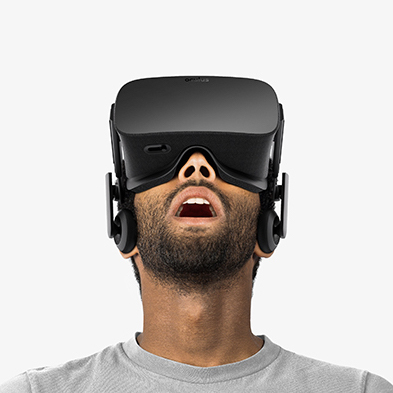
\includegraphics[width=3.0cm]{./figs/device-oculus.jpg}
	}
	\subfigure[Sony PlayStation]{
		\label{Sony PlayStation}
        %\caption{Sony PlayStation VR}
		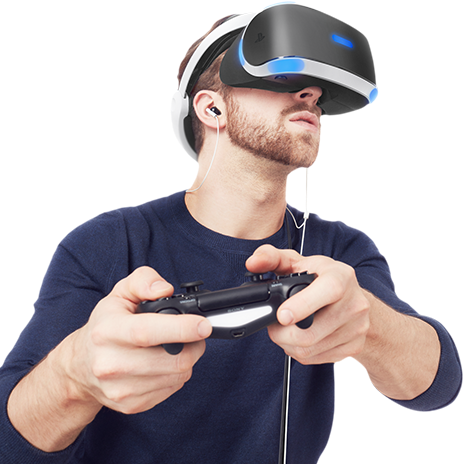
\includegraphics[width=3.0cm]{./figs/device-sony-vr.png}
	}
    \subfigure[HTC Vive]{
        \label{HTC Vive}
        %\caption{HTC Vive}
        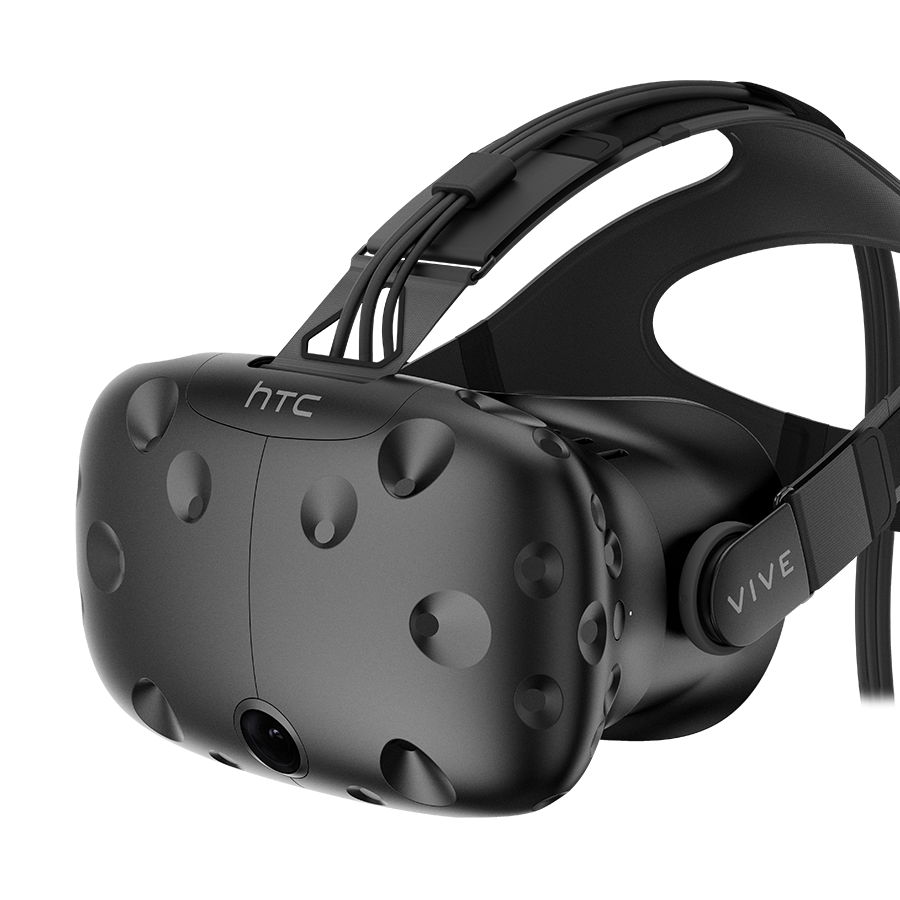
\includegraphics[width=3.0cm]{./figs/device-htc-vive-large.png}
    }
    \subfigure[Samsung Gear]{
        \label{Samsung Gear}
        %\caption{Samsung Gear VR}
        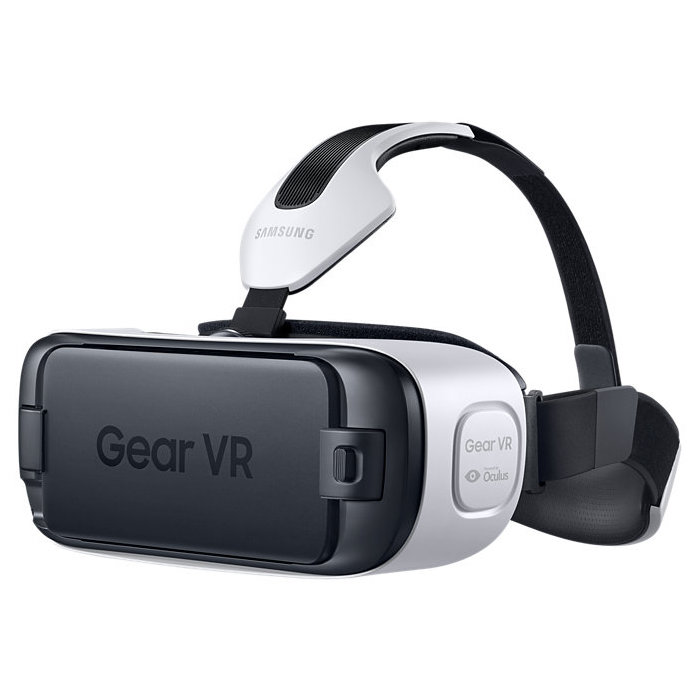
\includegraphics[width=3.0cm]{./figs/device-sumsung-gear-vr.jpeg}
    }
	\caption{Popular VR Hardwares}
	\label{VR products}
\end{figure}

Virtual reality and augmented reality have different use cases, technologies, and market opportunities, so it's important to distinguish between the two. Virtual reality immerses a user in an imagined or replicated world (like videogames, movies, or flight simulation) or simulates presence in the real world (like watching a sporting event live). Example of hardware players in VR are Oculus, Sony PlayStation VR, HTC Vive, and Samsung Gear VR shown in Fig.\ref{VR products}. Augmented reality overlays digital imagery onto real world. Examples of hardware players in AR are Microsoft HoloLens, Google Glass, and Magic Leap as shown in Fig.\ref{AR products}. An easy way to differentiate between the two is that VR uses an opaque headset(which you cannot see through) to completely immerse the user in a virtual world whereas AR uses a clear headset so the users can see the real world and overlay infomation and imagery onto it.

%\begin{table}[htbp]
%	\renewcommand{\arraystretch}{1.3}
%	\caption{Comparison between AR and VR}
%	\label{comparision between AR and VR}
%	\centering
%	\begin{tabular}{|m{2.0cm}|m{5.0cm}|m{5.0cm}|}
%	\hline
%	 & Augmented Reality & Virtual Reality\\
%	\hline
%	Attribute    & Both Virtual and Reality & Virtual\\
%	\hline
%	Enviroment   & Real (Physical) & Virtual\\
%	\hline
%	Scenarios    & Demonstrations, Architechure, Designing & Video Games Related\\
%	\hline
%	Interactions & Move, Rotate, Scale and Manipulate the 3D object in real world & Move, Rotate and Scale 3D object in virtual world\\
%    \hline
%    Techniques   & Display, Calibration, Tracking and Interaction & Same with AR\\
%    \hline
%	\end{tabular}
%\end{table}

While VR and AR can have different use cases, we view both technologies as driving the broader trend of HMDs as a computing form factor. Whether for consumer use or enterprise use, both VR and AR technology have the challenge of convincing the world that the value proposition is high enough to add another device to the current state of offerings in desktops, notebooks, tablets, and smartphones. Further, both VR and AR are gesture-based where the controls are largely driven by head and hand movements; while we view these gesture-based controls as intuitive this will serve as a new way to navigate the computing enviroment.

\begin{figure}[!hbp]
	\centering
    \subfigure[HoloLens]{
		\label{HoloLens}
        %\caption{Oculus VR}
		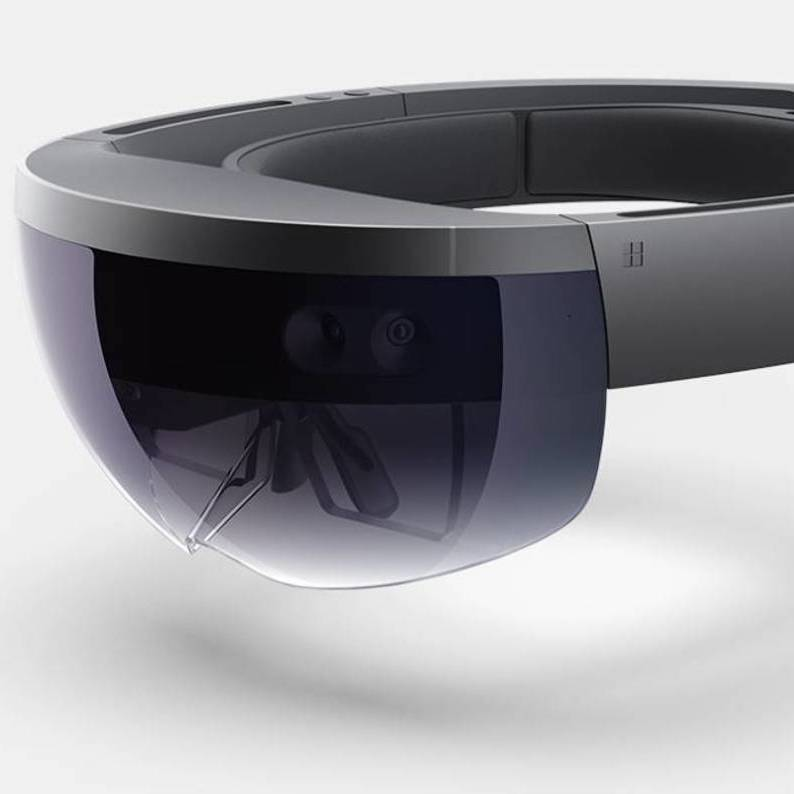
\includegraphics[width=4.0cm]{./figs/device-hololens.jpg}
	}
	\subfigure[Google Glass]{
		\label{Google Glass}
        %\caption{Sony PlayStation VR}
		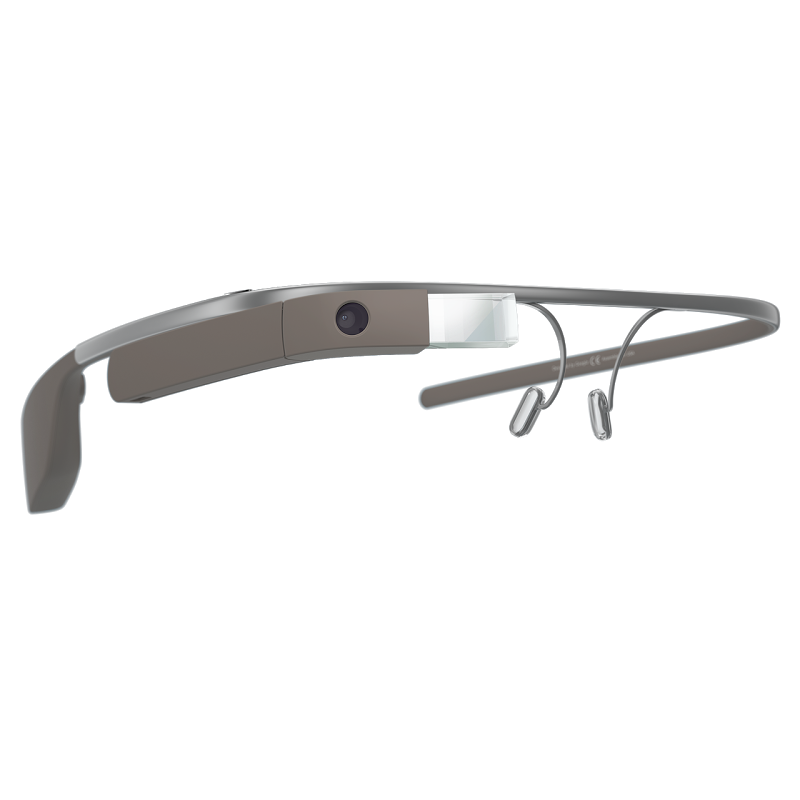
\includegraphics[width=4.0cm]{./figs/device-google-glass.png}
	}
    \subfigure[Magic Leap]{
        \label{Magic Leap}
        %\caption{Sony PlayStation VR}
        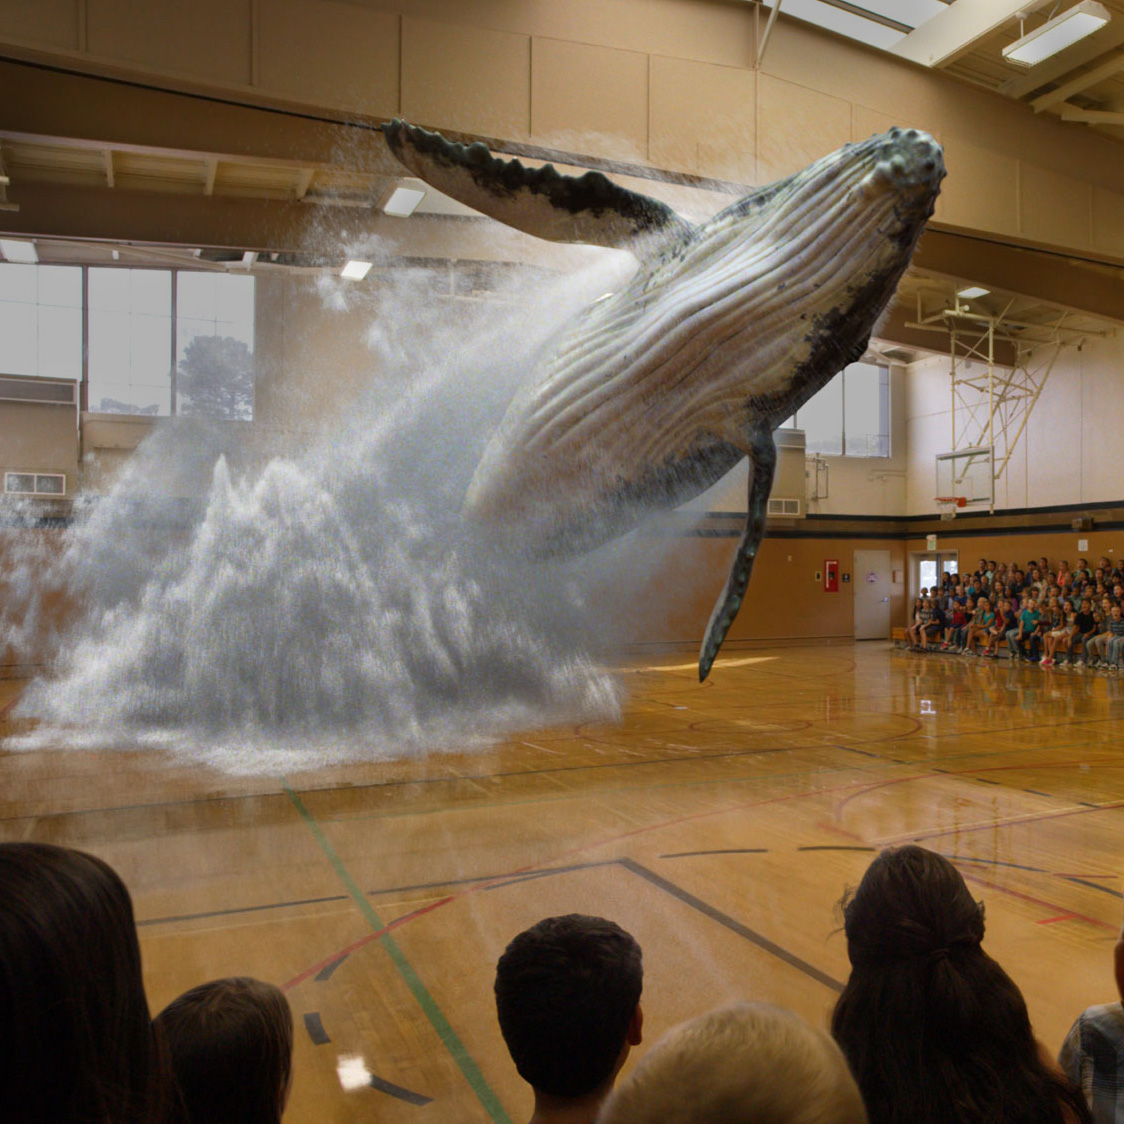
\includegraphics[width=4.0cm]{./figs/device-magic-leap.jpg}
    }
	\caption{Popular AR Hardwares and solution}
	\label{AR products}
\end{figure}


The rest of this survey is organised as follows: in Section 2, this survey will introduce the history of augmented reality and virtual reality; in Section 3, this paper will illustrate the supporting techniques; in the next section, this paper will show their industrial influences; in section 5 and 6, this paper will analyse the opportunities and challenges of AR/VR.  method and its local applications to both respiratory motion monitoring and ultrasonic image fusion. Finally, this paper gives briefly discussion and conclusion in Section 7.% Structure of this paper

\section{Evolution}  %% History of Techniques

\subsection{Brief History of AR}
The first AR prototypes (Fig. \ref{the first head-mounted-device}), created by computer graphics pioneer Ivan Sutherland and his students at Harvard University and the University of Utah, appeared in the 1960s and used a see-through to present 3D graphics\cite{tamura2001mixed}. During the 1970s and 1980s, mobile devices were introduced. For decades, researchers are paving the way for wearable computing techniques until early 1990s the term "augmented reality" was proposed\cite{caudell1992augmented}. By the late 1990s, as AR became a distinct field of research, several conferences on AR began.

%A small group of researchers at U.S. Air Force's Armstrong Laboratory, the NASA Ames Research Center, the Massachusetts Institute of Technology, and the University of North Carolina at Chapel Hill continued research during the 1970s and 1980s. During this time mobile devices like the Sony Walkman (1979), digital watches and personal digital organisers were introduced. This paved the way for wearable computing [103, 147] in the 1990s as personal computers became small enough to be worn at all times. Early palmtop computers include the Psion I (1984), the Apple Newton MessagePad (1993), and the Palm Pilot (1996). Today, many mobile platforms exist that may support AR, such as personal digital assistants (PDAs), tablet PCs, and mobile phones.

\begin{figure}[!hbp]
	\centering
	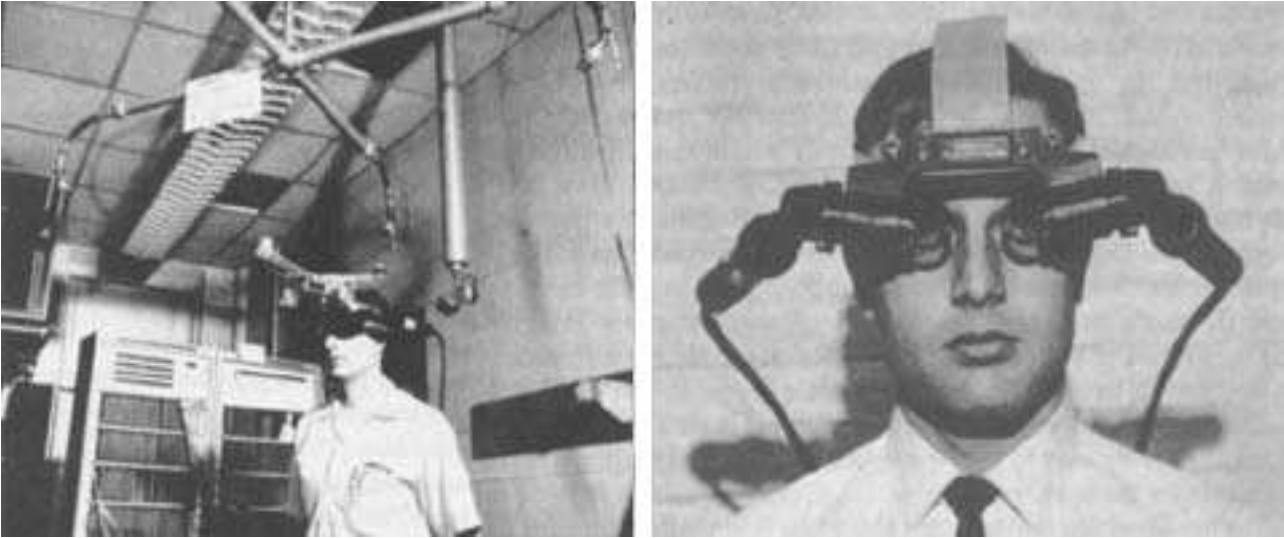
\includegraphics[width=12cm]{./figs/device-first-hmd.png}
	\caption{The world's first head-mounted display with the "Sword of Damocles"\cite{tamura2001mixed}}
	\label{the first head-mounted-device}
\end{figure}

In the 21st century, augmented reality makes great progress. In 2000, Bruce H. Thomas develops ARQuake, the first outdoor mobile AR game, demonstrating it in the International Symposium on Wearable Computers. In 2004, Trimble Navigation and the Human Interface Technology Laboratory demostrated the Outdoor helmet-mounted AR system. In 2012, AR gaming platform Lyteshot was launched that could utilizes smartglasses for game data. In 2013, Google announces an open beta test of its Google Glass augmented reality glasses. In 2015, Microsoft announces Windows Holographic and the HoloLens augmented reality headset. The headset utilizes various sensors and a processing unit to blend high definition "holograms" with the real world. Then, Niantic released Pokémon Go for iOS and Android in July 2016. The game quickly became one of the most used applications and has brought augmented reality to the mainstream.\cite{schepercenter}
%, including the International Workshop and Symposium on Augmented Reality, the International Symposium on Mixed Reality, and the Designing Augmented Reality Environments workshop. Organisations were formed such as the Mixed Reality Systems Laboratory2 (MRLab) in Nottingham and the Arvika consortium3 in Germany. Also, it became possible to rapidly build AR applications thanks to freely available software toolkits like the ARToolKit. In the meantime, several surveys appeared that give an overview on AR advances, describe its problems, classify and summarise developments [17, 19, 28]. By 2001, MRLab finished their pilot research, and the symposia were united in the International Symposium on Mixed and Augmented Reality4 (ISMAR), which has become the major symposium for industry and research to exchange problems and solutions.

%For anyone who is interested and wants to get acquainted with the field, this survey provides an overview of important technologies, applications and limitations of AR systems. After describing technologies that enable an augmented reality experience in Section 2, we review some of the possibilities of AR systems in Section 3. In Section 4 we discuss a number of common technological challenges and limitations regarding human factors. Finally, we conclude with a number of directions that the authors envision AR research might take.

\subsection{Brief History of VR}

Virtual reality was first coined in 1987 by Jaron Lanier, founder of the visual programming lab where several VR devices like the Data Glove, the Eye Phone and the Audio Sphere were invented. In the 1990s, the public gradually had access to VR devices, although household ownership of cutting edge virtual reality was still far out of reach. The Virtuality Group launched a range of arcade games and machines. The Lawnmower Man movie introduced the concept of virtual reality to a wider audience. In 1995, Nintendo Virtual Boy (originally known as VR-32) was launched and it was be the first ever portable console that could display true 3D graphics.

% Before 1980s, virtual reality was not well known. The concept of virtual reality was popularized in mass media by movies such as Brainstorm (1983) and The Lawnmower Man. In 1990s, most ideas about VR remained theoretical due to the limited computing power available at the time. The extremely high cost of the technology made it impossible for consumers to adopt. When the Internet became widely available, this became the technology focus for most people. The VR industry mainly provided VR devices for medical, flight simulation, automobile industry design, and military training purposes from 1970 to 1990.

The first fifteen years of the 21st century has seen major, rapid advancement in the development of virtual reality. Computer technology, especially small and powerful mobile technologies, have exploded while prices are constantly driven down. Recently Google have released interim virtual reality products such as the Google Cardboard. Samsung have taken this concept further with products such as the Galaxy Gear, which is mass produced and contains "smart" features such as gesture control. Developer versions of final consumer products have also been available for a few years, so there has been a steady stream of software projects creating content for the immanent market entrance of modern virtual reality.

%The rise of smartphones with high-density displays and 3D graphics capabilities has enabled a generation of lightweight and practical virtual reality devices. The video game industry has continued to drive the development of consumer virtual reality unabated. Depth sensing cameras sensor suites, motion controllers and natural human interfaces are already a part of daily human computing tasks.

It seems clear that 2016 will be a key year in the virtual reality industry. Multiple consumer devices that seem to finally answer the unfulfilled promises made by virtual reality in the 1990s will come to market at that time. These include the pioneering Oculus Rift, which was purchased by social media giant Facebook in 2014 for the staggering sum of \$2BN. An incredible vote of confidence in where the industry is set to go. When the Oculus Rift releases in 2016 it will be competing with products from Valve corporation and HTC, Microsoft as well as Sony Computer Entertainment. These heavyweights are sure to be followed by many other enterprises, should the market take off as expected.

%In 2001, SAS3 or SAS Cube became the first PC based cubic room, developed by Z-A Production (Maurice Benayoun, David Nahon), Barco, Clarté, installed in Laval France in April 2001. The SAS library gave birth to Virtools VRPack. By 2007, Google introduced Street View, a service that shows panoramic views of an increasing number of worldwide positions such as roads, indoor buildings and rural areas. It also features a stereoscopic 3D mode, introduced in 2010.[24] In 2010, Palmer Luckey, who later went on to found Oculus VR, designed the first prototype of the Oculus Rift. This prototype, built on a shell of another virtual reality headset, displayed only 2-D images and was noticeably cumbersome to wear. However, it boasted a 90-degree field of vision that was previously unseen anywhere in the market at the time. This initial design would later serve as a basis from which the later designs came.[25]

%In 2013, Nintendo filed a patent for the concept of using VR technology to produce a more realistic 3D effect on a 2D television. A camera on the TV tracks the viewer's location relative to the TV, and if the viewer moves, everything on the screen reorients itself appropriately. "For example, if you were looking at a forest, you could shift your head to the right to discover someone standing behind a tree."[26] In July 2013, Guild Software's Vendetta Online was widely reported as the first MMORPG to support the Oculus Rift,[27][28] making it potentially the first persistent online world with native support for a consumer virtual reality headset. Since 2013, there have been several virtual reality devices that seek to enter the market to complement Oculus Rift to enhance the game experience. One, Virtuix Omni, is based on the ability to move in a three dimensional environment through an omnidirectional treadmill.

%On March 25, 2014, Facebook purchased a company that makes virtual reality headsets, Oculus VR, for \$2 billion.[29] In that same month, Sony announced Project Morpheus (its code name for PlayStation VR), a virtual reality headset for the PlayStation 4 video game console.[30] Google announces Cardboard, a do-it-yourself stereoscopic viewer for smartphones. The user places her smartphone in the cardboard holder, which she wears on her head. In 2015, the Kickstarter campaign for Gloveone, a pair of gloves providing motion tracking and haptic feedback, was successfully funded, with over \$150,000 in contributions.[31]

%In February–March 2015, HTC partnered with Valve Corporation announced their virtual reality headset HTC Vive and controllers, along with their tracking technology called Lighthouse, which utilizes "base stations" mounted to the wall above the user's head in the corners of a room for positional tracking of the Vive headset and its motion controllers using infrared light.[32][33][34][35] The company announced its plans to release the Vive to the public in April 2016 on December 8, 2015.[36][37] Units began shipping on April 5, 2016.[38]

%In July 2015, OnePlus became the first company to launch a product using virtual reality.[39] They used VR as the platform to launch their second flagship device the OnePlus 2, first viewable using an app on the Google Play Store,[40] then on YouTube.[41] The launch was viewable using OnePlus Cardboard, based on the Google's own Cardboard platform. The whole VR launch had a runtime of 33 minutes, and was viewable in all countries. Also in 2015, Jaunt, a startup company developing cameras and a cloud distribution platform, whose content will be accessible using an app, reached \$100 million in funding from such sources as Disney and Madison Square Garden.[42] On April 27, 2016, Mojang announced that Minecraft is now playable on the Gear VR.[43] Minecraft is still being developed for the Oculus Rift headset but a separate version was released to the Oculus Store for use with the Gear VR. This version is similar to the Pocket Edition of Minecraft.

%\section{Enabling Technology}


\section{Applications \& Industry} %% effect on traditional industries
\subsection{Create New Markets}
Some advanced haptic systems in the 2010s now include tactile information, generally known as force feedback in medical, video gaming and military training applications. Some VR systems used in video games can transmit vibrations and other sensations to the user via the game controller. Virtual reality also refers to remote communication environments which provide a virtual presence of users with through telepresence and telexistence or the use of a virtual artifact (VA), either through the use of standard input devices such as a keyboard and mouse, or through multimodal devices such as a wired glove or omnidirectional treadmills. The immersive environment can be similar to the real world in order to create a lifelike experience—for example, in simulations for pilot or combat training, which depict realistic images and sounds of the world, where the normal laws of physics apply (e.g., in flight simulators), or it can differ significantly from reality, such as in VR video games that take place in fantasy settings, where gamers can use fictional magic and telekinesis powers.

%%As we discuss in more detail in the use cases section of this report, we currently see AR geared towards serving business use cases, VR having both consumer and business applications, and some areas where the two overlap. For instance, most video game development is in VR right now, but Microsoft HololLens is also creating AR games such as Minecraft.


\subsection{Reform Old Industries}
%%Education and training
%Entertainment and games
%Artistic Creation
%Medical Application
%Manufacturing
%Military
%Collaboration
%Navigation
%Tourism
Both AR and VR have the potential to not only create new markets but also disrupt existing ones. Nine cases for AR/VR technology are emerging: videogames, live events, video entertainment, retail, real estate, education, healthcare, engineer, and military (Fig.\ref{AR VR applications}).

\begin{figure}[!hbp]
	\centering
    \subfigure[Education and training]{
		\label{Education and training}
		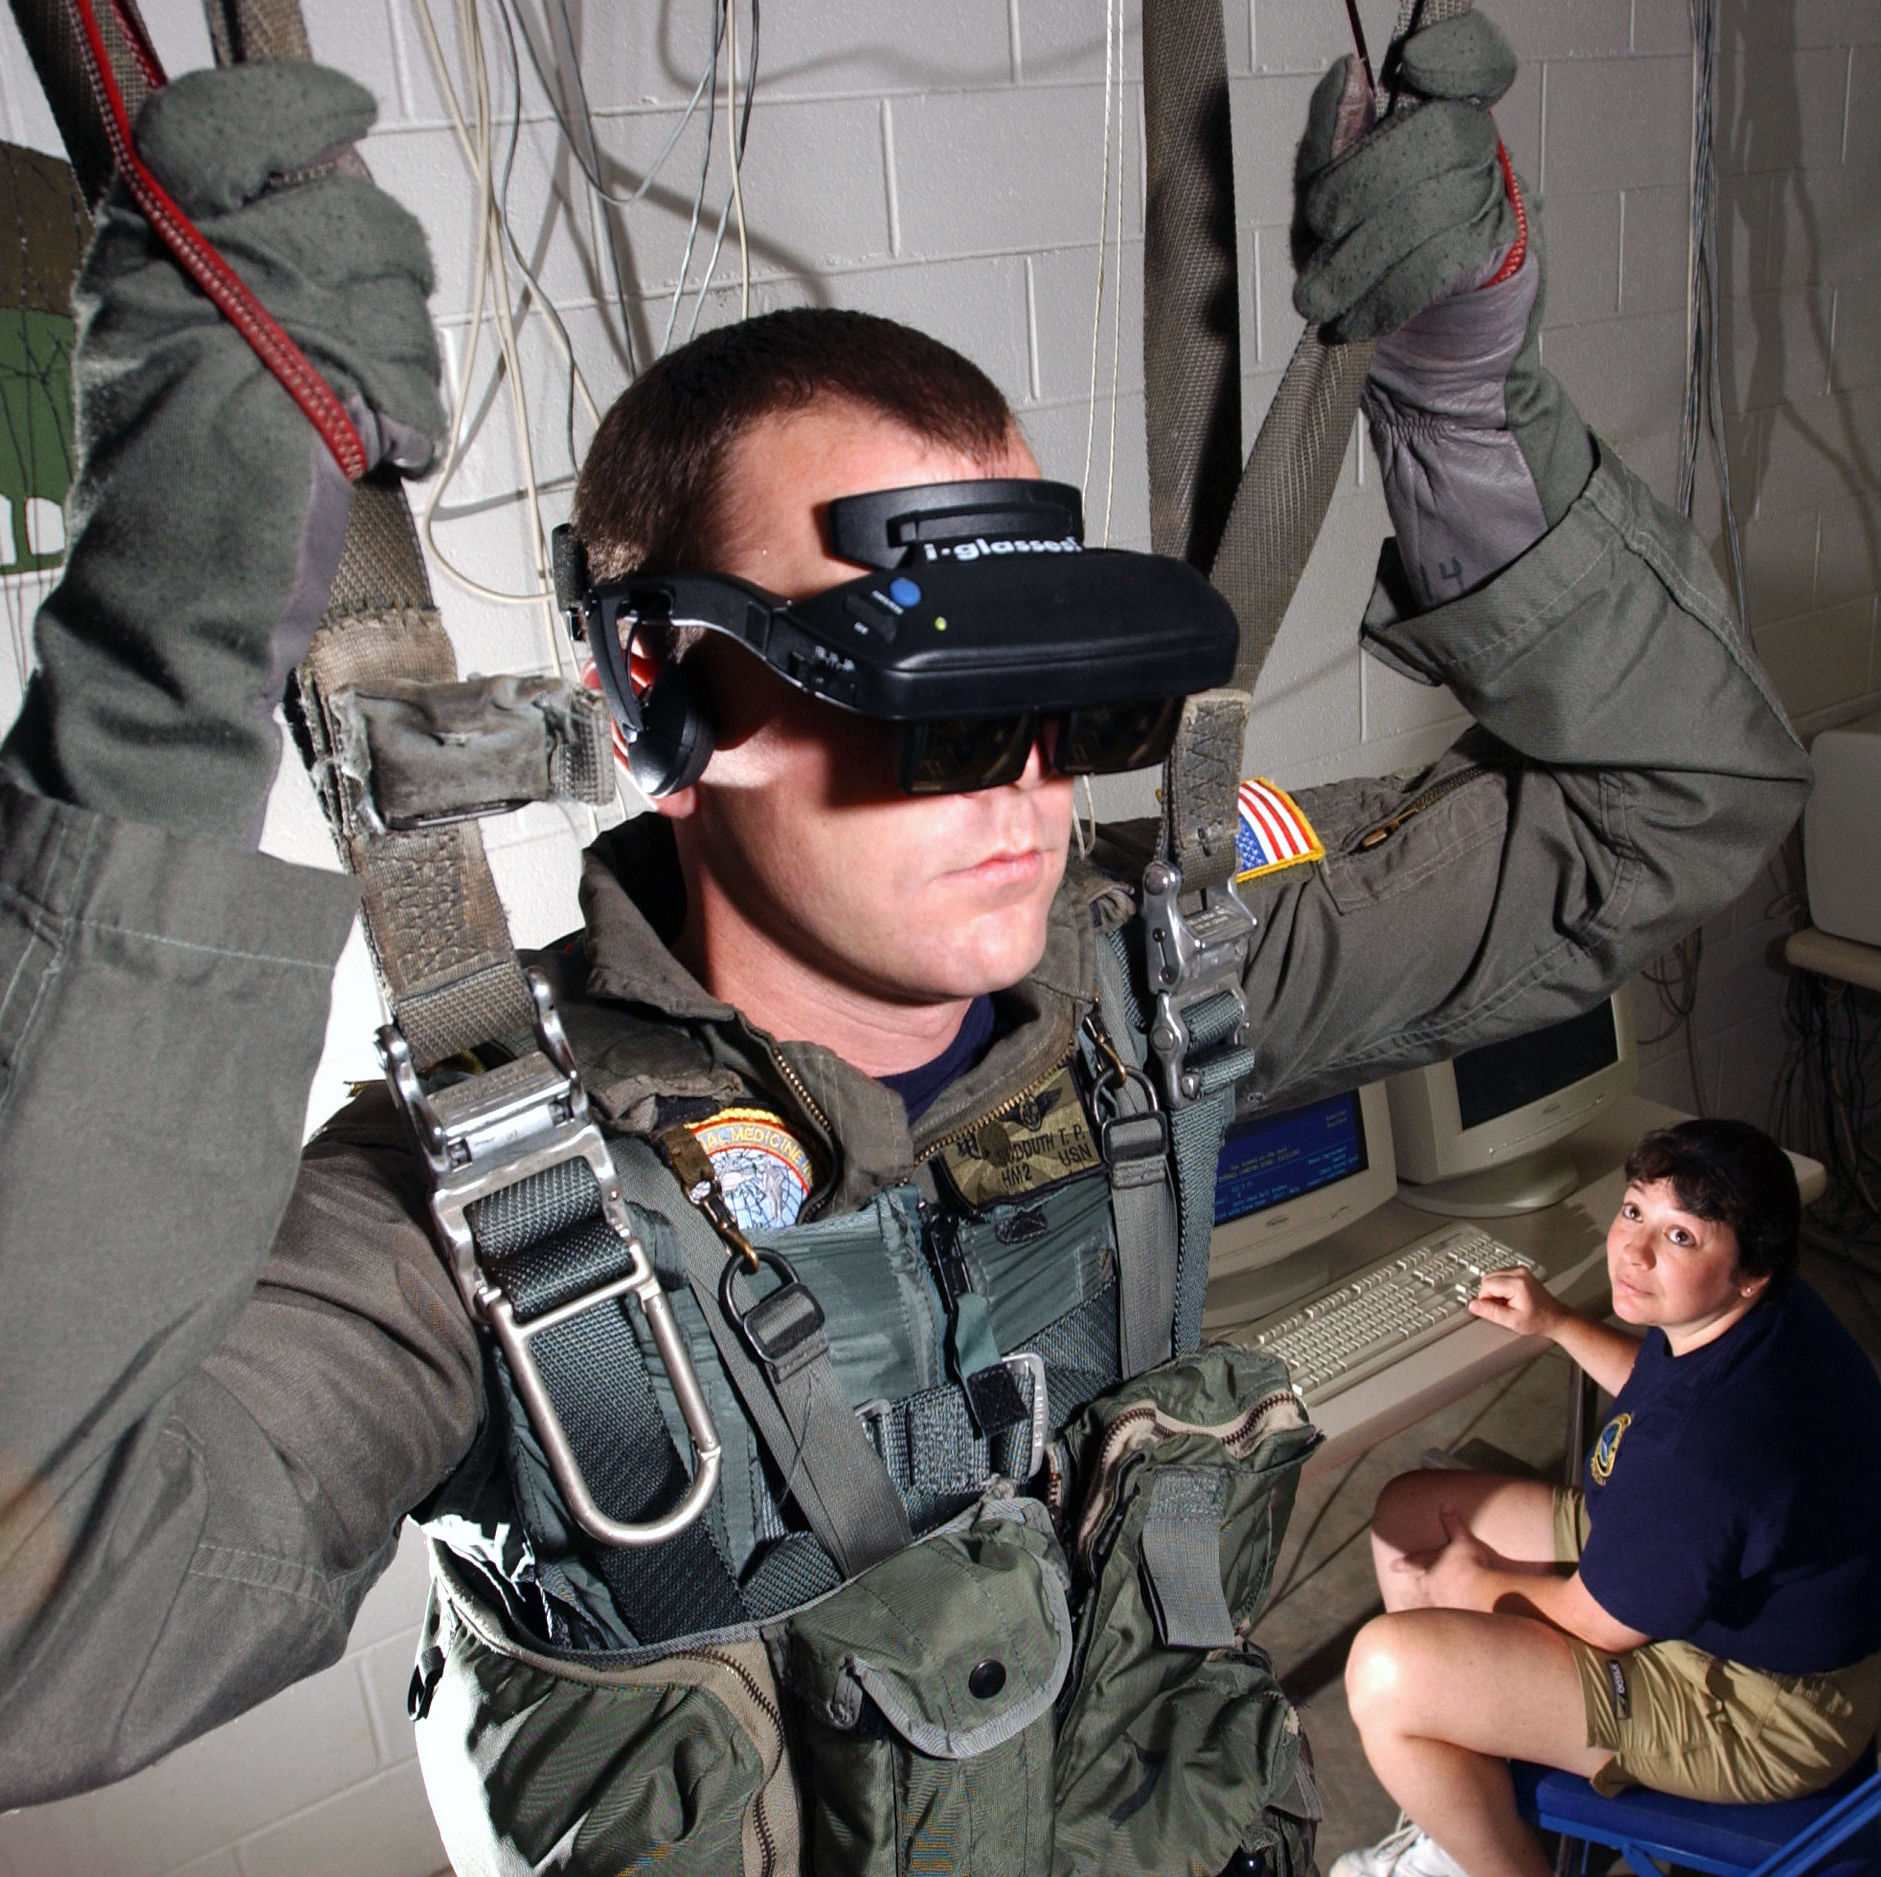
\includegraphics[width=3.0cm]{./figs/application-training.jpg}
	}
	\subfigure[Entertainment]{
		\label{Entertainment}
		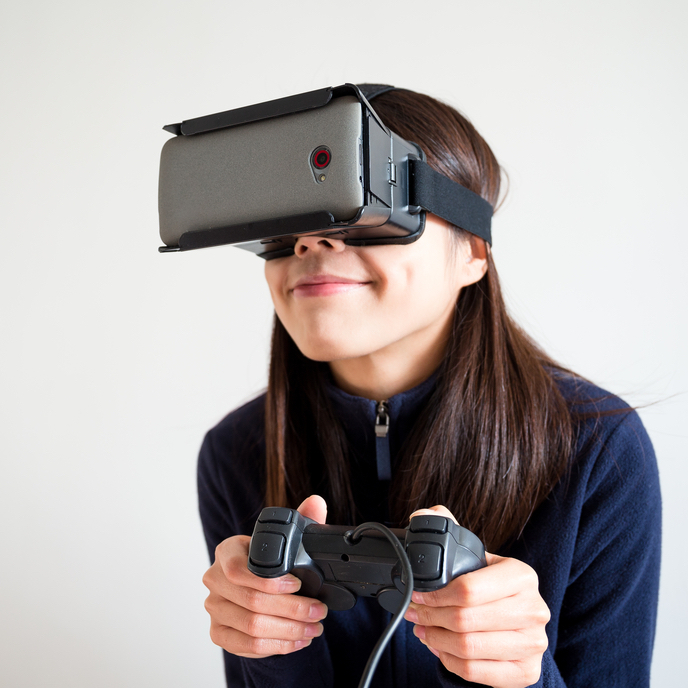
\includegraphics[width=3.0cm]{./figs/application-gaming.jpg}
	}
    \subfigure[Medical Application]{
        \label{Medical Application}
        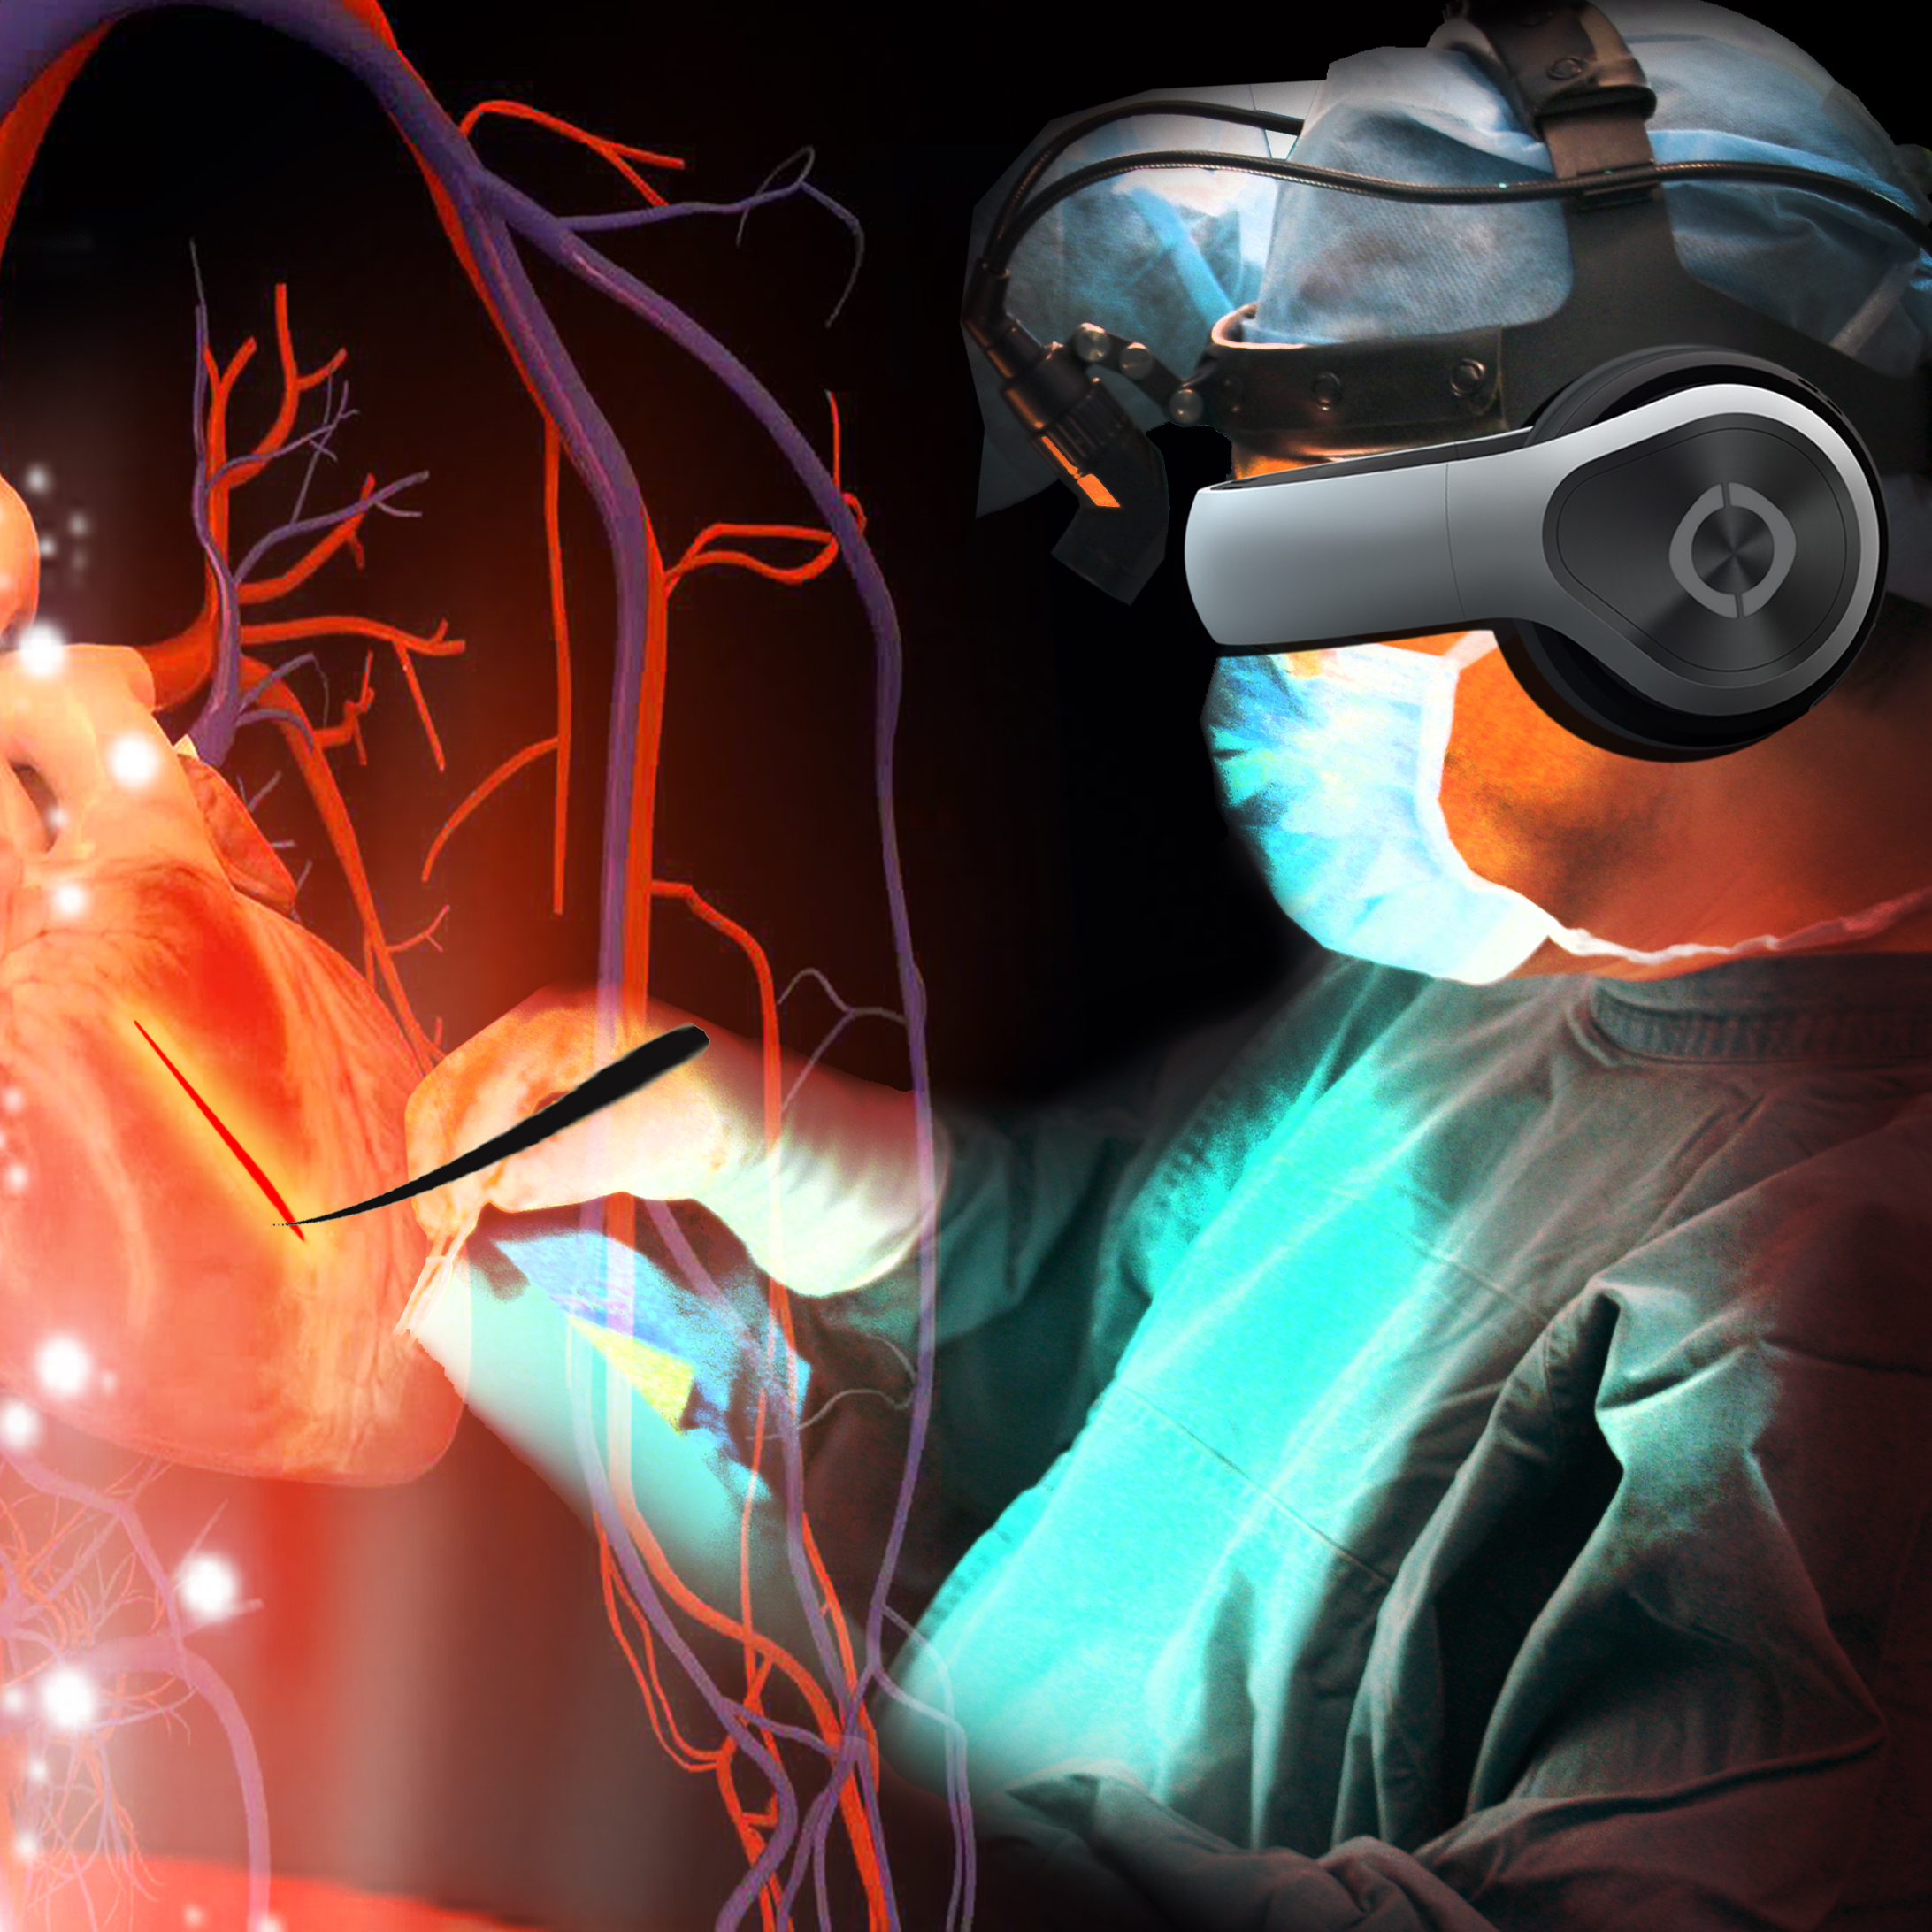
\includegraphics[width=3.0cm]{./figs/application-medical.jpg}
    }
    \subfigure[Manufacturing]{
        \label{Manufacturing}
        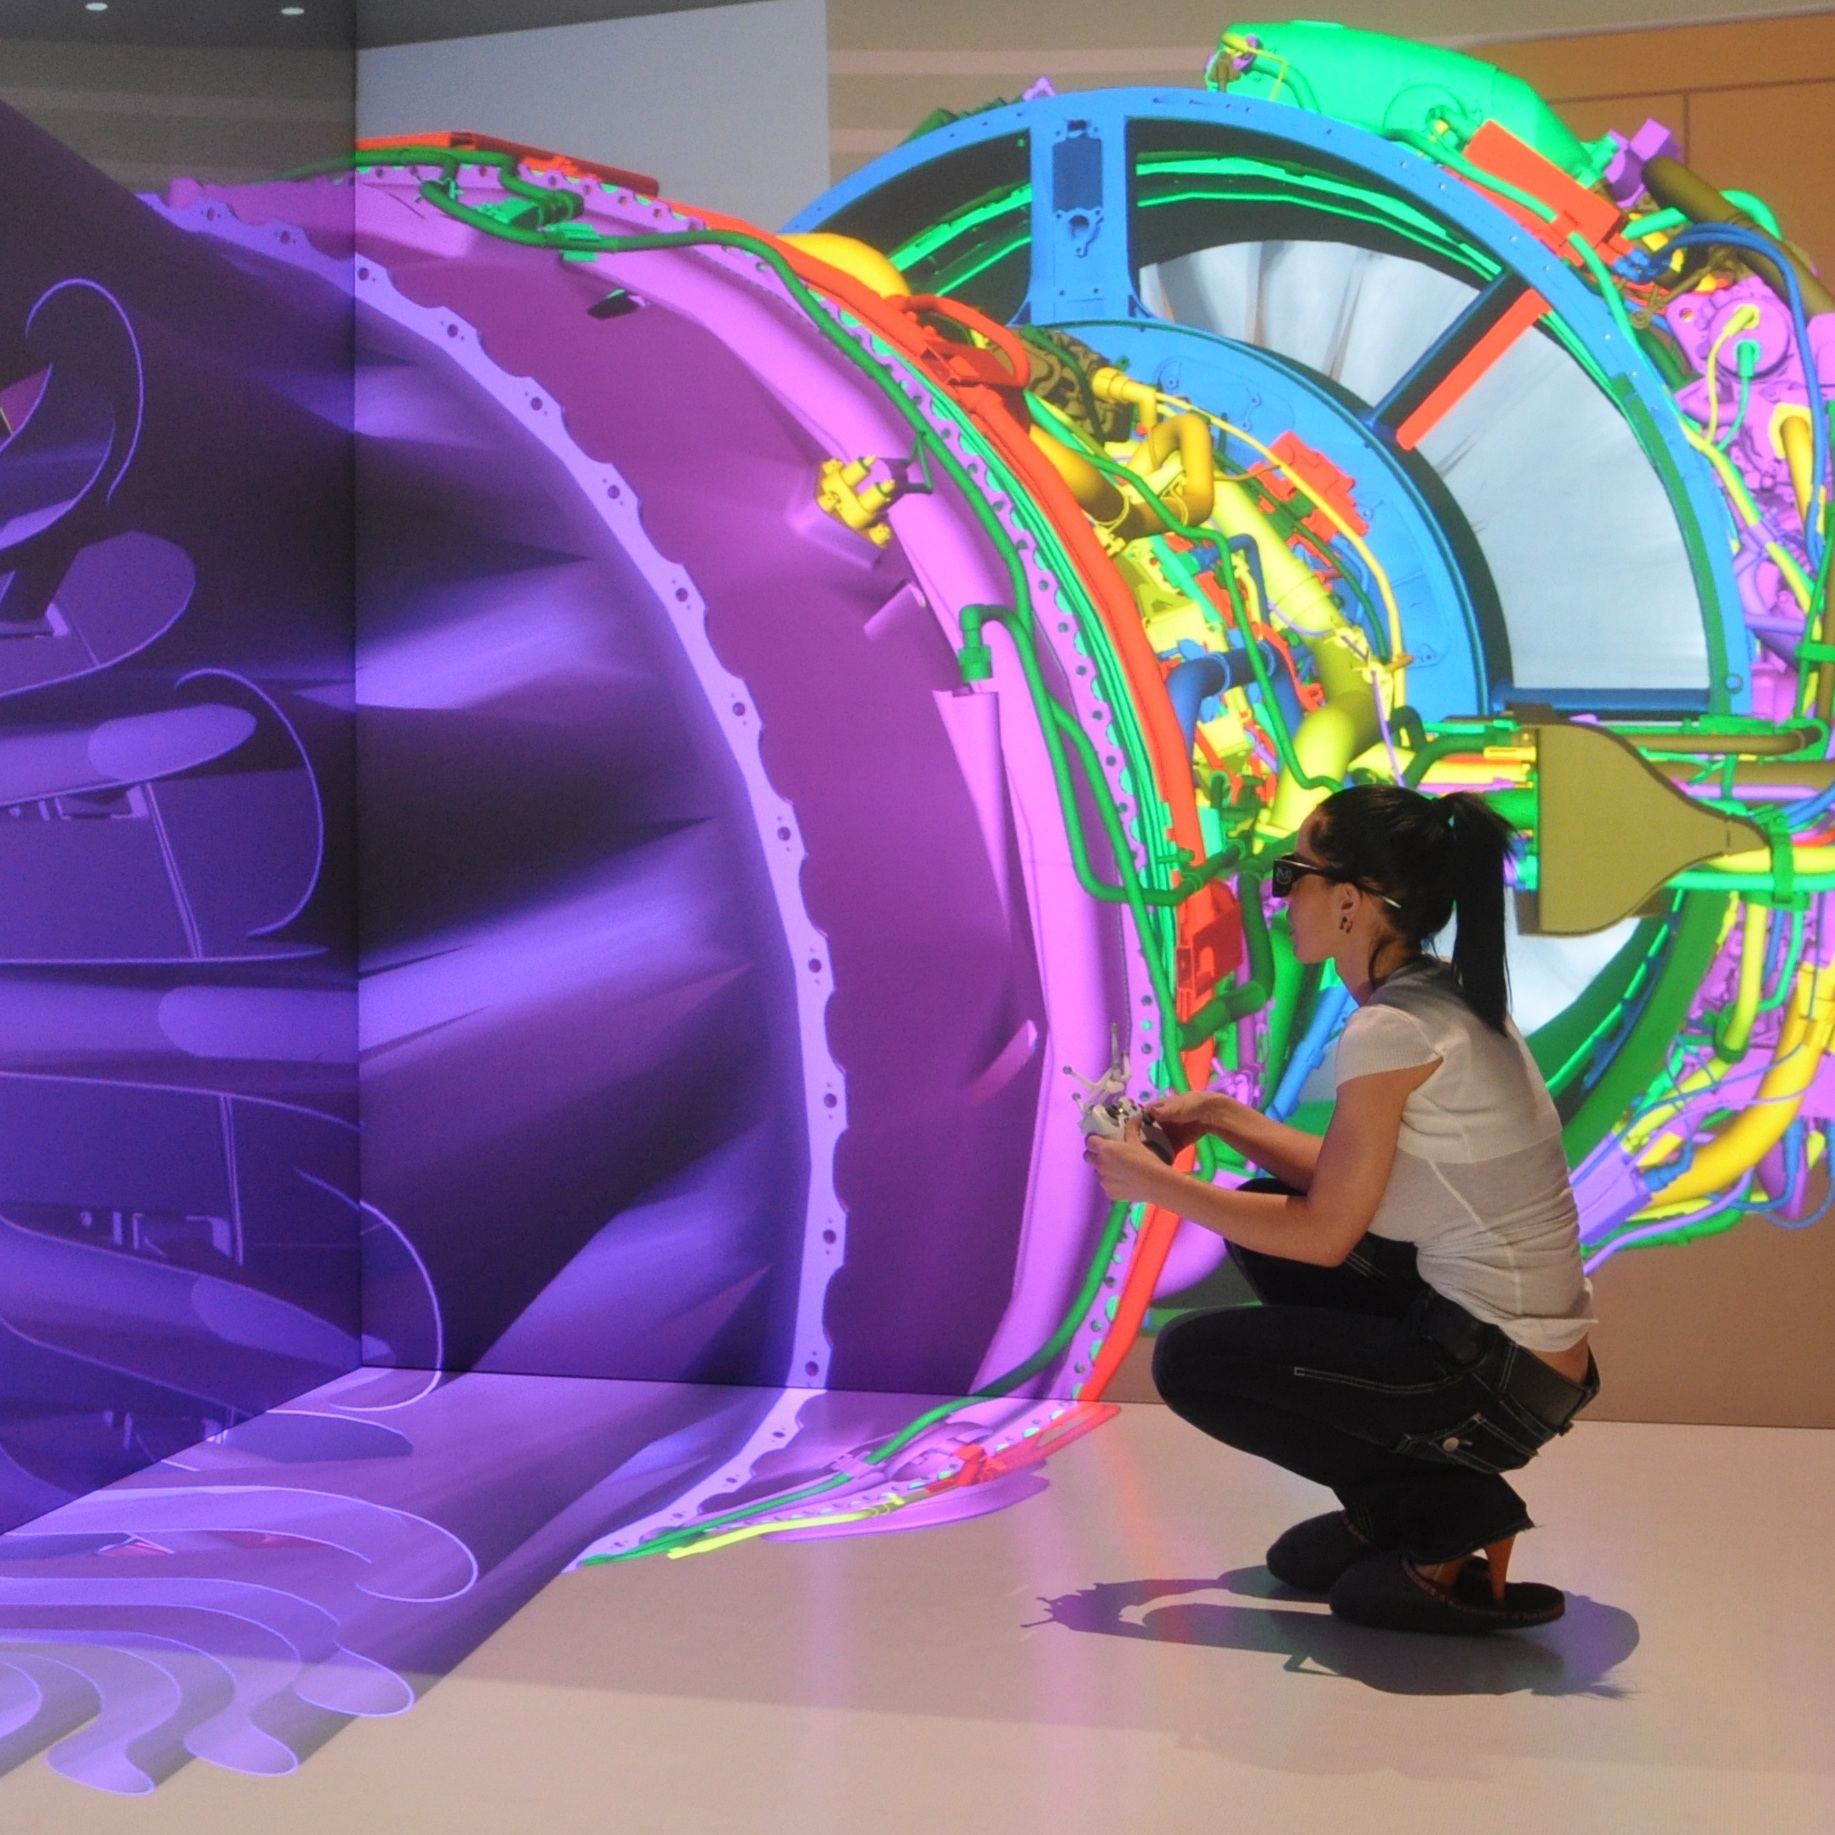
\includegraphics[width=3.0cm]{./figs/application-manufacturing.jpg}
    }
    \subfigure[Tourism]{
        \label{Military}
        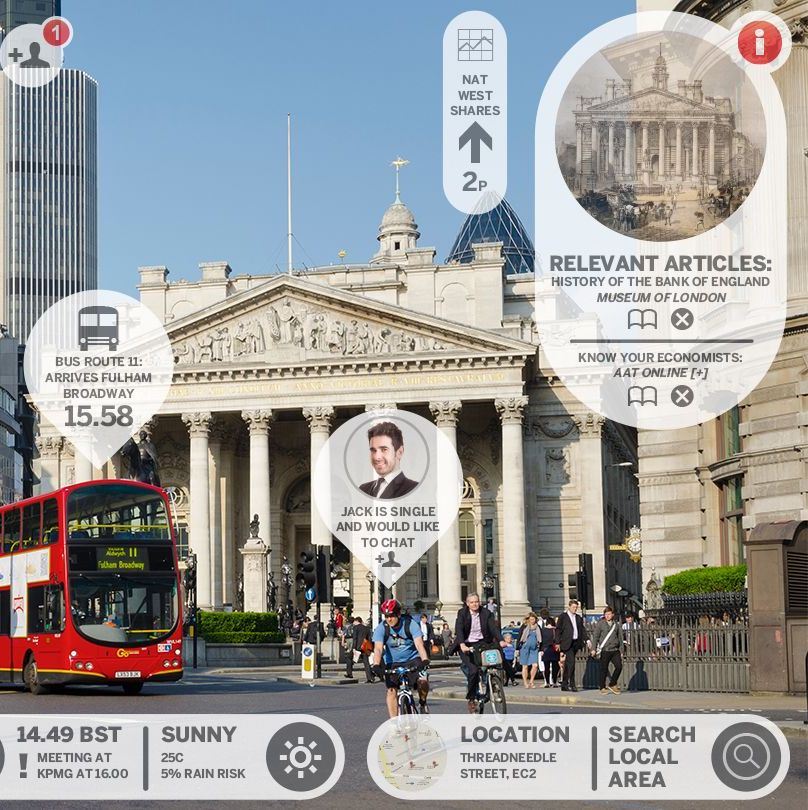
\includegraphics[width=3.0cm]{./figs/application-tourism.jpg}
    }
    \subfigure[Collaboration]{
        \label{Collaboration}
        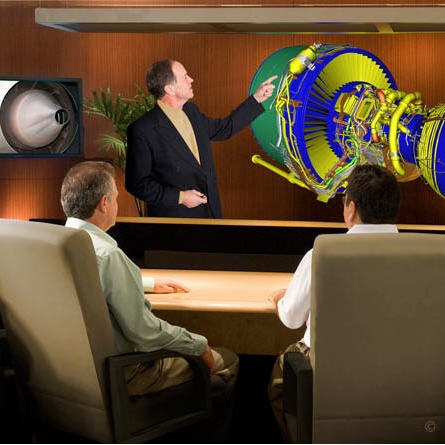
\includegraphics[width=3.0cm]{./figs/application-collaboration.jpg}
    }
    \subfigure[Design]{
        \label{Military}
        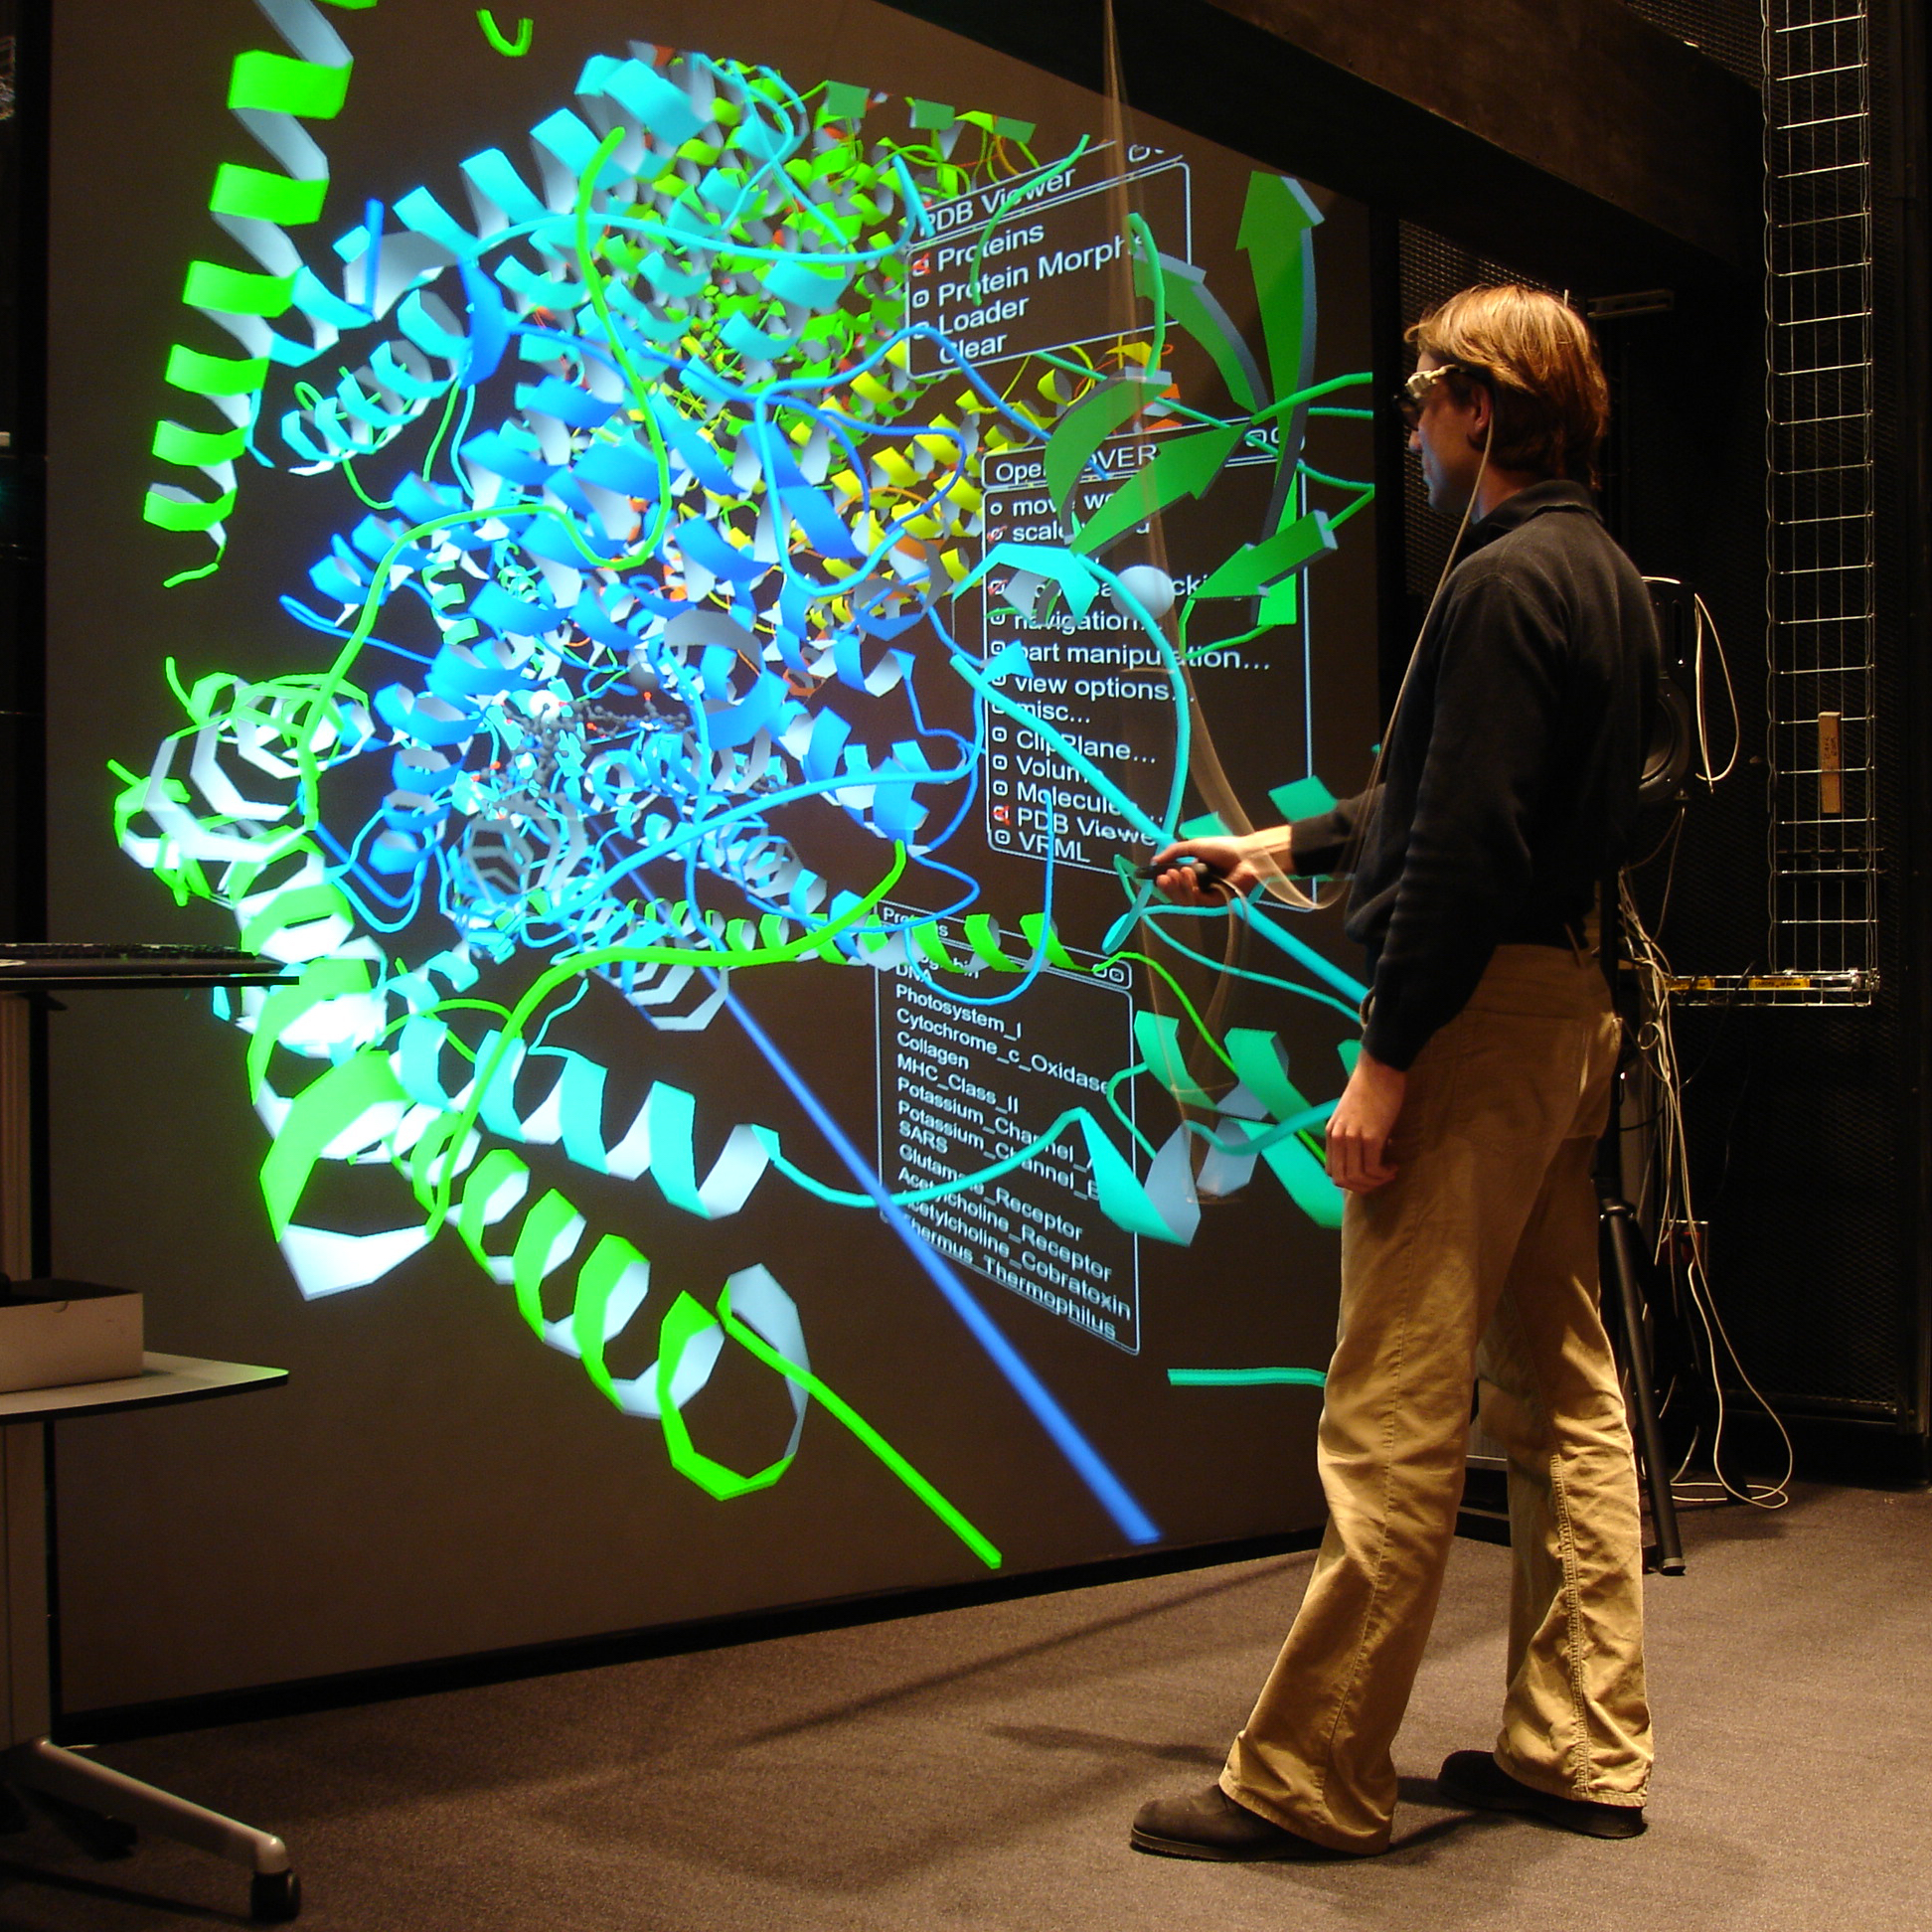
\includegraphics[width=3.0cm]{./figs/application-design.jpg}
    }
    \subfigure[Navigation]{
        \label{Collaboration}
        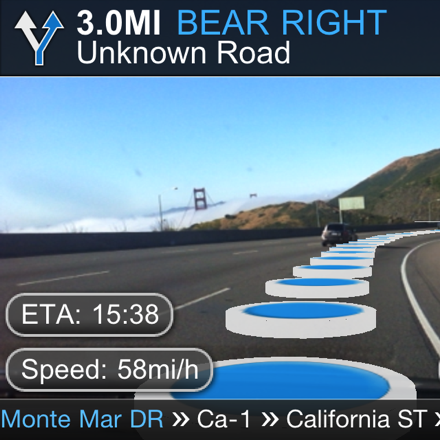
\includegraphics[width=3.0cm]{./figs/application-navigation.jpg}
    }
	\caption{Popular applications of AR or VR}
	\label{AR VR applications}
\end{figure}

According to the prediction from GoldmanSach 2016, videogames, live events, and video entertainment are the only 3 cases that are entirely driven by the consumer and make up ~60\% of total AR/VR revenue assumptions for 2025. The remaining ~40\% is driving by enterprise and public sector spend with the largest revenue generating use cases in engineering, healthcare, and real estate. Some use cases are specific to VR, some use cases are specific to AR, and some cases overlap. The report indicates that AR technology still needs to mature, especially in display technology and the real-time processing and calibration of real-world physical enviroment. As AR technology matures, we see stronger enterprise use cases emergeing especially considering AR enables you to see your physical environment whereas VR completely blocks it.

%% 插图
\begin{figure}[!hbp]
	\centering
    \subfigure[]{
		\label{2025 VR/AR estimates by use case}
		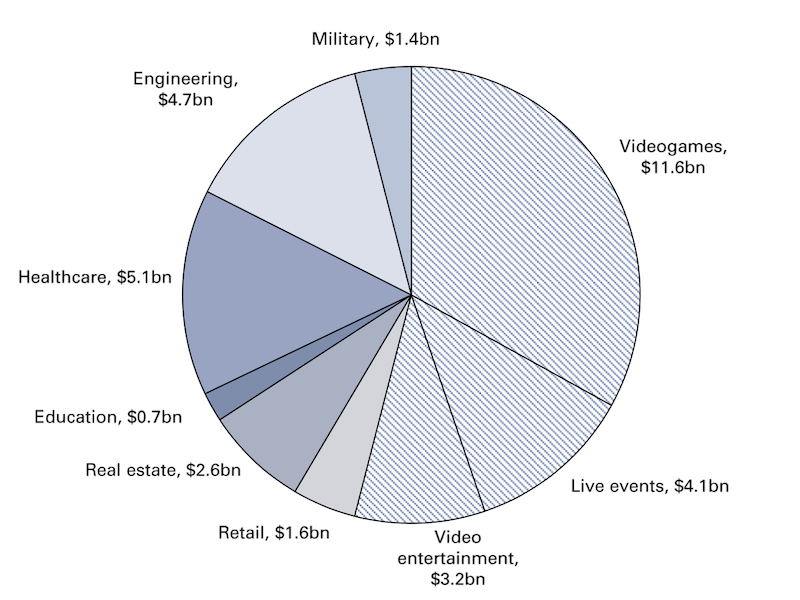
\includegraphics[width=6.0cm]{./figs/2025_estimate_by_use_cases.png}
	}
	\subfigure[]{
		\label{2025 software estimates by AR and VR}
		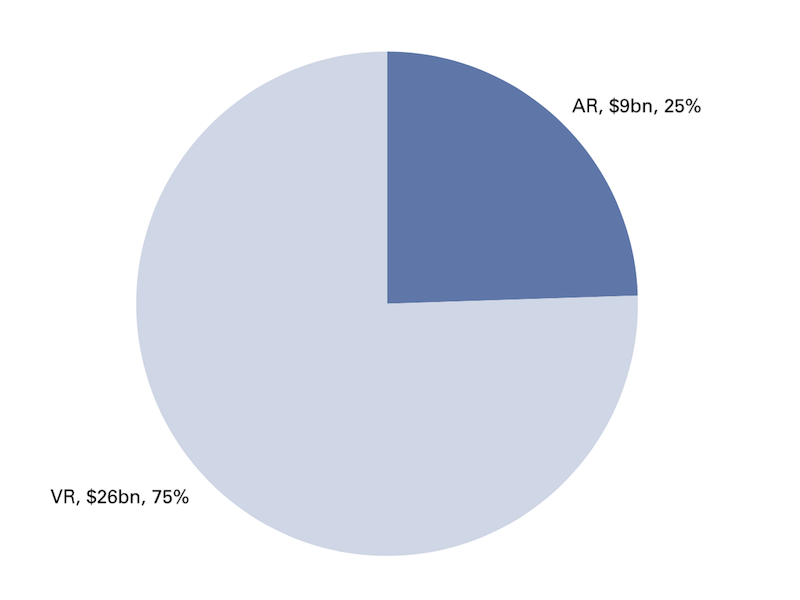
\includegraphics[width=6.0cm]{./figs/2025_software_estimate_by_vr_and_ar.png}
	}
	\caption{(a)Consumer-driven use cases in videogames, live events and video driving ~60\% of software spend with the remainder from enterprise and public sector; (b)VR use cases driving 75\% of our software estimate; as AR technology matures we expect more enterprise use cases to emerge}
	\label{Predition from Goldman Sachs Global Investment Research}
\end{figure}



%%\section{Future} %% oppurtunity
%%\subsection{Market Prediction}
%%\subsection{Impacts on Conventional Industries}



\section{Challenges} %% challenge
%%The display technology, The real-time processing, The calibration of real-world physical environment
\subsection{The Limitations of Augmented Reality}
AR faces technical challenges regarding for example binocular (stereo) view, high resolution, colour depth, luminance, contrast, field of view, and focus depth. However, before AR becomes accepted as part of user's everyday life, just like mobile phones and personal digital assistants (PDAs), issues regarding intuitive interfaces, costs, weight, power usage, ergonomics, and appearance must also be addressed. A number of limitations, some of which have been mentioned earlier, are categorised here.

%\subsubsection{Portability and Outdoor Use}
%Most mobile AR systems mentioned in this survey are cumbersome, requiring a heavy backpack to carry the PC, sensors, display, batteries, and everything else. Connections between all the devices must be able to withstand outdoor use, including weather and shock, but universal serial bus (USB) connectors are known to fail easily. However, recent developments in mobile technology like cell phones and PDAs are bridging the gap towards mobile AR.
%Optical and video see-through displays are usually unsuited for outdoor use due to low brightness, contrast, resolution, and field of view. However, recently developed at MicroVision, laser-powered displays offer a new dimension in head-mounted and hand-held displays that overcomes this problem.
%Most portable computers have only one CPU which limits the amount of visual and hybrid tracking. More generally, consumer operating systems are not suited for real-time computing, while specialised real-time operating systems don't have the drivers to support the sensors and graphics in modern hardware.

%\subsubsection{Tracking and Calibration (auto)}
%Tracking in unprepared environments remains a challenge but hybrid approaches are becoming small enough to be added to mobile phones or PDAs. Calibration of these de- vices is still complicated and extensive, but this may be solved through calibration-free or auto-calibrating approaches that minimise setup requirements. The latter use redundant sensor information to automatically measure and compensate for changing calibration parameters [19].
%Latency A large source of dynamic registration errors are system delays [19]. Techniques like precalculation, temporal stream matching (in video see-through such as live broadcasts), and prediction of future viewpoints may solve some delay. System latency can also be scheduled to reduce errors through careful system design, and prerendered images may be shifted at the last instant to compensate for pantilt motions. Similarly, image warping may correct delays in 6DOF motion (both translation and rotation).

%\subsubsection{Depth Perception}
%One difficult registration problem is accurate depth perception. Stereoscopic displays help, but additional problems including accommodation-vergence conflicts or low resolution and dim displays cause object to appear further away than they should be [52]. Correct occlusion ameliorates some depth problems [138], as does consistent registration for different eyepoint locations [158].
%In early video see-through systems with a parallax, users need to adapt to vertical displaced viewpoints. In an experiment by Biocca and Rolland [35], subjects exhibit a large overshoot in a depth-pointing task after removing the HMD.
%\subsubsection{Overload and Over-reliance}

Aside from technical challenges, the user interface must also follow some guidelines as not to overload the user with information while also preventing the user to overly rely on the AR system such that important cues from the environment are missed\cite{vlahakis2001archeoguide}. At BMW, Bengler and Passaro use guidelines for AR system design in cars, including orientation on the driving task, no moving or obstructing imagery, add only information that improves driving performance, avoid side effects like tunnel vision and cognitive capture, and only use information that does not distract, intrude or disturb given different situations.

%\subsubsection{Social Acceptance}

Getting people to use AR may be more challenging than expected, and many factors play a role in social acceptance of AR ranging from unobtrusive fashionable appearance (gloves, helmets, etc.) to privacy concerns. These fundamental issues must be addressed before AR is widely accepted\cite{hughes2005mixed}.

\subsection{The Limitations of Virtual Reality}
%\subsubsection{Health and Safty Considerations}
There are certain health and safety considerations of virtual reality. For example, a number of unwanted symptoms have been caused by prolonged use of virtual reality,\cite{kela2006accelerometer} and these may have slowed proliferation of the technology. Most virtual reality systems come with consumer warnings. Virtual reality sickness (also known as cybersickness) occurs when a person's exposure to a virtual environment causes symptoms that are similar to motion sickness symptoms.\cite{kim2009simulated} The most common symptoms are general discomfort, headache, stomach awareness, nausea, vomiting, pallor, sweating, fatigue, drowsiness, disorientation, and apathy.\cite{seungjun2006reliable} Other symptoms include postural instability and retching.

%Virtual reality sickness is different from motion sickness in that it can be caused by the visually-induced perception of self-motion; real self-motion is not needed. It is also different from simulator sickness; non-virtual reality simulator sickness tends to be characterized by oculomotor disturbances, whereas virtual reality sickness tends to be characterized by disorientation.

%\subsubsection{Social and Philosophical}
In addition, there are social and philosophical considerations and implications associated with the use of virtual reality. There has been an increase in interest in the potential social impact of new technologies, such as virtual reality. Mychilo S. Cline's book Power, Madness, and Immortality: The Future of Virtual Reality, argues that virtual reality will lead to a number of important changes in human life and activity.\cite{stricker2001augmented} He argues that virtual reality will be integrated into daily life and activity, and will be used in various human ways. Another such speculation has been written up on how to reach ultimate happiness via virtual reality.\cite{kotranza2008virtual} He also argues that techniques will be developed to influence human behavior, interpersonal communication, and cognition. As we spend more and more time in virtual space, there would be a gradual "migration to virtual space", resulting in important changes in economics, worldview, and culture.

%In the book The Metaphysics of Virtual Reality by Michael R. Heim, seven different concepts of virtual reality are identified: simulation, interaction, artificiality, immersion, telepresence, full-body immersion, and network communication.

%Philosophical implications of VR are discussed in books, including Philip Zhai's Get Real: A Philosophical Adventure in Virtual Reality (1998) and Digital Sensations: Space, Identity and Embodiment in Virtual Reality (1999), written by Ken Hillis.

%\subsubsection{Technical Difficulties}
Virtual reality technology faces a number of challenges, most of which involve motion sickness and technical matters. Users might become disoriented in a purely virtual environment, causing balance issues; computer latency might affect the simulation, providing a less-than-satisfactory user experience; the complicated nature of head-mounted displays and input systems such as specialized gloves and boots may require specialized training to operate, and navigating the non-virtual environment (if the user is not confined to a limited area) might prove dangerous without external sensory information. There are areas of VR that need solutions, such as 3D audio, haptics, body tracking, and input. However, 3D audio effects exist in games and simulate the head-related transfer function of the listener (especially using headphones). There have been rising concerns that with the advent of virtual reality, some users may experience virtual reality addiction.

\section{Discuss \& Conclusion}

Fundamentally, virtual/augmented reality creates a new and even more intuitive way to interact with a computer. In the world of virtual/augmented reality, the controls of the computer become what we are already familiar with through gestures and graphics. VR/AR also gives us wider field of view, where the concept of virtual desktop is no longer confined by the size of a physical display screen on our desktop or in the palm of our hands. Given this attribute of ease of use and the multiple use cases across VR/AR, we see the potential for technology to emerge from vertical specific use cases to a broader computing platform. Meanwhile, virtual/augmented reality faces a bunch of challenges, including not only technical problems, but nontechnical problems such as social acceptance, health considerations and even philosophical issues.

\label{}

%% The Appendices part is started with the command \appendix;
%% appendix sections are then done as normal sections
%% \appendix

%% \section{}
%% \label{}

%% If you have bibdatabase file and want bibtex to generate the
%% bibitems, please use
%%
%%  \bibliographystyle{elsarticle-num}
%%  \bibliography{<your bibdatabase>}

%% else use the following coding to input the bibitems directly in the
%% TeX file.

\section*{Reference}

\bibliographystyle{elsarticle-num}
\bibliography{elsarticle-template-num}

\end{document}
\endinput
%%
%% End of file `elsarticle-template-num.tex'.
